\documentclass[tikz,border=10pt,transparent]{standalone}
\usepackage{tikz-feynman}
\usepackage{xcolor}

\definecolor{cream}{HTML}{F2EDE4}
\definecolor{terracotta}{HTML}{B8693C}
\definecolor{mutedteal}{HTML}{7FAF9A}

\begin{document}

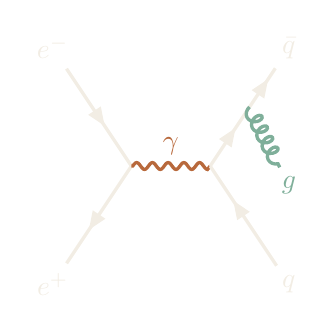
\begin{tikzpicture}
  \begin{feynman}
    \vertex (i1) at (-1,  1.5) {\textcolor{cream}{\(e^{-}\)}};
    \vertex (i2) at (-1, -1.5) {\textcolor{cream}{\(e^{+}\)}};
    \vertex (a)  at ( 0,  0);
    \vertex (b)  at ( 1,  0);
    \vertex (m)  at ( 1.5, 0.75);
    \vertex (f1) at ( 2,  1.5) {\textcolor{cream}{\(\bar{q}\)}};
    \vertex (f2) at ( 2, -1.5) {\textcolor{cream}{\(q\)}};
    \vertex (g1) at ( 2, -0.25) {\textcolor{mutedteal}{\(g\)}};

    \diagram* {
      (i1) -- [fermion, very thick, color=cream] (a),
      (i2) -- [anti fermion, very thick, color=cream] (a),
      (a)  -- [photon, very thick, color=terracotta,
               edge label=\textcolor{terracotta}{\(\gamma\)}] (b),
      (b)  -- [fermion, very thick, color=cream] (m) -- [fermion, very thick, color=cream] (f1),
      (b)  -- [anti fermion, very thick, color=cream] (f2),
      (m)  -- [gluon, very thick, color=mutedteal] (g1),
    };
  \end{feynman}
\end{tikzpicture}

\end{document}